\begin{figure}
  \centering
  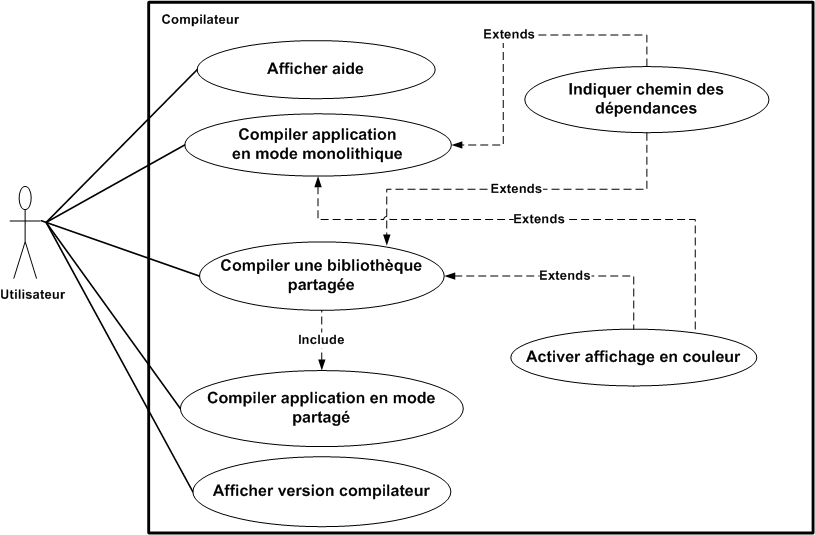
\includegraphics[scale=0.8]{../res/stb/UseCase_F.jpg}
  \caption{\textbf{Cas d'utilisations du compilateur kawa.}}
\end{figure}

%Cas d'utilisation
\subsection{Cas d'utilisation EF\_1}
\fiche
{Afficher l'aide}                    % Nom du cas d'utilisation
{Utilisateur du compilateur}                               % Acteurs concernés
{                                                % Description
  le compilateur affiche 
   la liste des options du compilateur sur la sortie standard à travers une ligne de commande.
}
{
  L'ordre de priorité entre le commutateur de help (-h ou -\hspace{0.1mm}-help) et le commutateur de version (-v ou -\hspace{0.1mm}-version) est définit par le commutateur en premier paramètre. Le commutateur -h/-\hspace{0.1mm}-help est le premier paramètre obligatoirement.
}                                                % Préconditions
{Commutateur de ligne de commande :kawac -h ou -\hspace{0.1mm}-help }                             % Evénements déclenchants
{L'aide a été affichée correctement et la main est redonnée à l'utilisateur pour entrer d'autres commutateurs.}                       % Conditions d'arrêt
% {0.6}{../res/stb/usecase2_flot_event.png}      % Diagramme
{} % acteur(s)
{} % system
{} % flot exceptionsb
 % fin usecase EF_1

\subsection{Cas d'utilisation EF\_2}
\fiche
{Compiler une application en mode monolithique}                    % Nom du cas d'utilisation
{Utilisateur du compilateur}                               % Acteurs concernés
{                                                % Description
  L'utilisateur introduit un ensemble de modules (classe/interface)
  kawa afin de les précompiler et de générer une application sous forme d'un seul exécutable.
}
{
	Afin de permettre la compilation dans ce mode monolithique il faut:
	\begin{itemize}
  	\item Indiquer l’emplacement des fichiers sources de l'application.
  	\item Introduire le commutateur  \textbf {-m}  en premier paramètre dans la ligne de commande permettant la compilation.
  	\item L'absence des deux commutateurs (-h ou -\hspace{0.1mm}-help) et (-v ou -\hspace{0.1mm}-version) en premier paramètre.
  	\end {itemize}
}                                                % Préconditions
{

Afin de pouvoir lancer la compilation dans ce mode l'utilisateur  doit: 
\begin{itemize}
  	\item Indiquer au moins un module (une classe avec une méthode main qui constitue le point d'entrée d'une application).
  	\item Introduire une ligne de commande avec un commutateur d'action: kawac -m filessources.
 \end {itemize}

}    % Evénements déclenchants
{
	\begin{itemize}
  	\item La compilation s'est terminée sans erreurs dans ces différentes étapes d’analyses.
  	\item La production d’un unique fichier exécutable sous le format d'ELF  qui ne dépend d'aucune bibliothèque kawa ainsi que le nom du fichier exécutable correspond au nom du module contenant la méthode main.
\end {itemize}
  
}  % Conditions d'arrêt
%{0.6}{../res/stb/usecase2_flot_event.png} 		 % Diagramme
{                                                % Flots d'exceptions
  
}
{} % system
{
La compilation peut être interrompue pour divers raisons, on cite:

	\begin{itemize}
  	\item \textbf {EF\_2\_EXC\_1}: Le fichier de sortie n'a pu être créé.
  	\item  \textbf {EF\_2\_EXC\_2}: Le code source d'un des modules de l'application comporte une erreur syntaxique, l'erreur rencontrée pendant cette étape d'analyse est renvoyée sur la sortie standard du compilateur.
  	\item \textbf {EF\_2\_EXC\_3}: Le code source d'un des modules (classe/interface) dont dépend le programme est introuvable. Un message renvoyé par le compilateur indique le nom du (ou des) module(s) manquants sur la sortie standard.
  	\item \textbf {EF\_2\_EXC\_4}: Le code source d'un des modules de l'application comporte une erreur sémantique, exemple : l'incompatibilité de type statique lors d'une opération d'affectation.
  	\item \textbf {EF\_2\_EXC\_5}: Aucun des modules indiqués ne comporte le point d'entrée (main).
  	\item \textbf {EF\_2\_EXC\_6}: Plusieurs méthodes main ont été trouvées parmi les classes indiquées dans le source, le compilateur renvoie la liste des points d'entrée trouvés sur la sortie standard.
  	\end {itemize}
 } % flot exceptions
% Fin de la fiche du cas d'utilisation 1.


%Cas d'utilisation 2
\subsection{Cas d'utilisation EF\_3}
\fiche
{Compiler une application en mode partagé}                    % Nom du cas d'utilisation
{Utilisateur du compilateur}                               % Acteurs concernés
{                                                % Description
  L’utilisateur introduit un ensemble de sources kawa
 qui peuvent appeler des bibliothèques externes. Le compilateur doit être capable de trouver les bibliothèques pour les utiliser ou bien  de les recompiler si nécessaire. La différence entre ce mode et le mode monolithique est que le fichier exécutable et la bibliothèque sont indépendants avant le lancement de l’application, et peuvent être maintenus séparément à l'encontre du mode monolithique qui génère un seul exécutable regroupant le tout. Pour les bibliothèques partagées l'édition des liens se fait à l’exécution (au moment du lancement du programme) au contraire des bibliothèques statiques où l'édition des liens se fait dans la phase de compilation. 
}
{
	Afin de permettre la compilation dans ce mode il faut:
	\begin{itemize}
  	\item Spécifier l’emplacement des fichiers sources de l'application.
  	\item L'absence du commutateur  \textbf {-m}  en premier paramètre.
  	\item L'absence des deux commutateurs (-h ou -\hspace{0.1mm}-help) et (-v ou -\hspace{0.1mm}-version) en premier paramètre.
  	\end {itemize}

	
}                                                % Préconditions
{

Afin de pouvoir lancer la compilation dans ce mode l'utilisateur  doit: 
\begin{itemize}
  	\item Indiquer au moins un module (une classe avec une méthode main qui constitue le point d'entrée d'une application).
  	\item Introduire une ligne de commande sans commutateur d'action (fonctionnement par défaut): kawac filessources [options].
 \end {itemize}
 L'utilisateur peut éventuellement compiler des fichiers des modules qui ne sont pas forcément en relation avec l'application à compiler.
}  % Evénements déclenchants
{
\begin{itemize}
  	\item La compilation s'est terminée sans erreurs dans ces différentes étapes d’analyses.
  	\item La production d’un unique fichier exécutable sous le format d'ELF et qui n'est pas sous l'extension (.so), le nom du fichier exécutable correspond au nom du module contenant la méthode main.
\end {itemize}
  	} % Conditions d'arrêt
%{0.6}{../res/stb/usecase2_flot_event.png} 		 % Diagramme
{                                                % Flots d'exceptions
  
}{} % system
{La compilation peut être interrompue pour divers raisons, on cite:

\begin{itemize}
  	\item \textbf {EF\_3\_EXC\_1}: Le fichier de sortie n'a pu être créé.
  	\item  \textbf {EF\_3\_EXC\_2}: Le code source d'un des modules de l'application comporte une erreur syntaxique, l'erreur rencontrée pendant cette étape d'analyse est renvoyée sur la sortie standard du compilateur.
  	\item \textbf {EF\_3\_EXC\_3}: Un module (classe ou interface) de l'application fait référence à un symbole externe introuvable, soit le paquetage externe contenant le symbole n'existe pas, ou bien il n'a pu être compiler à cause d'une erreur.
  	\item \textbf {EF\_3\_EXC\_4}: Le code source d'un des modules de l'application comporte une erreur sémantique, exemple : l'incompatibilité de type statique lors d'une opération d'affectation.
  	\item \textbf {EF\_3\_EXC\_5}: Aucun des modules indiqués ne comporte le point d'entrée (main).
  	\end {itemize}
 } % flot exceptions
% Fin de la fiche du cas d'utilisation 2.


%Cas d'utilisation
\subsection{Cas d'utilisation EF\_4}
\fiche
{Compiler une bibliothèques partagée}                      % Nom du cas d'utilisation
{Utilisateur du compilateur}                               % Acteurs concernés
{                                                % Description
    L'utilisateur peut compiler des bibliothèques partagée en introduisant le nom du paquetage contenant les sources de la bibliothèque, la bibliothèque elle même peut contenir des sous bibliothèques (sous paquetages), pour notre cas d'étude chaque sous paquetages aura son propre fichier (.so).

     Le compilateur produit du code compilé destiné à être partagé entre plusieurs différents programmes, l'extension de la bibliothèque produite sera (.so => Shared Object) qui est un unique fichier exécutable pour tout le paquetage. On ne peut compiler une bibliothèque partagée que dans un mode partagé avec la non présence cette fois ci de la méthode main.      
}
{
	Afin de permettre la compilation d'une bibliothèque partagée expicitement il faut:
	\begin{itemize}
  	\item Indiquer le nom du répertoire contenant les fichiers sources de la bibliothèque.
  	\item L'absence du commutateur \textbf {-m} en premier paramètre, pour indiquer qu'on est dans un mode paratgé.
  	\item L'absence des deux commutateurs (-h ou -\hspace{0.1mm}-help) et (-v ou -\hspace{0.1mm}-version) en premier paramètre.
  	\end {itemize}
}               % Préconditions
{
	Afin de pouvoir lancer la compilation de la bibliothèque l'utilisateur doit:
	\begin{itemize}
  	\item Indiquer le nom du paquetage contenant les sources de la bibliothèque.
  	\item Introduire la ligne de commande sans les commutateurs d'actions: kawac filessources [options].
  	\end {itemize}

} % Evénements déclenchants
{{                                                % Flots d'exceptions
  
}{}
La compilation s'est terminée sans erreurs dans ces différentes étapes d'analyses et a comme résultats:
	\begin{itemize}
  	\item La production d'une bibliothèque dynamique dont le nom et l'emplacement correspondent à ceux du paquetage indiqué par l'utilisateur.
  	\item La bibliothèque va contenir les symboles de liaison pour tous les éléments publiques du paquetage.
  	\end {itemize}

} % Conditions d'arrêt
%{0.6}{../res/stb/usecase3_flot_event.png}     % Diagramme
{                                                % Flots d'exceptions
 
}{} % system
{	La compilation peut être interrompue pour divers raisons, on cite:
	\begin{itemize}
  	\item \textbf {EF\_4\_EXC\_1}: Le répertoire du paquetage est vide.
  	\item \textbf {EF\_4\_EXC\_2}: Erreur rencontrée lors de l'analyse syntaxique de l'un des modules du paquetage.
  	\item \textbf {EF\_4\_EXC\_3}: Erreur rencontrée lors de l'analyse sémantique de l'un des modules du paquetage.
  	\item \textbf {EF\_4\_EXC\_4}: Un module (classe ou interface) de la bibliothèque fait référence à un symbole externe introuvable, soit le paquetage externe contenant le symbole n'existe pas, ou bien il n'a pu être compiler à cause d'une erreur.

  	\item \textbf {EF\_4\_EXC\_5}: Un point d'entrée (main) a été trouvé dans l'un des modules du paquetage.
  	\end {itemize}

} % flot exceptions
% Fin de la fiche du cas d'utilisation 3.
%Cas d'utilisation
\subsection{Cas d'utilisation EF\_5}
\fiche
{Afficher la version du compilateur}                      % Nom du cas d'utilisation
{Utilisateur du compilateur}                               % Acteurs concernés
{                                                % Description
   
L'utilisateur peut savoir la version du compilateur avec le quel compile ses sources et ses bibliothèques  à travers un commutateur de ligne de commande.   
}
{
   L'odre de priorité entre le commutateur de help (-h ou -\hspace{0.1mm}-help) et le commutateur de version (-v ou -\hspace{0.1mm}-version) est définit par la première occurrence de l'un des deux commutateur i-e si nous avons un \textbf {-v} avant un \textbf {-h}, le compilateur annule tout le reste et affiche la version
}                                                % Préconditions
{Commutateur de ligne de commande:kawac -v ou -\hspace{0.1mm}-version}                             % Evénements déclenchants
{La version est affichée sur la sortie standard du compilateur.}                       % Conditions d'arrêt
%{0.6}{../res/stb/usecase3_flot_event.png}     % Diagramme
{                                                % Flots d'exceptions
 
}{} % system
{} % flot exceptions
% Fin de la fiche du cas d'utilisation 3.
%Cas d'utilisation
\subsection{Cas d'utilisation EF\_6}
\fiche
{Indiquer les chemins des dépendances}          % Nom du cas d'utilisation
{Utilisateur du compilateur}                               % Acteurs concernés
{                                                % Description
	Afin de permettre la définition  des schémas de dépendances entre le source de l'application et des modules externes (peuvent être des bibliothèques déjà compilées) il faut:   
	\begin{itemize}
  	\item Spécifier le chemin vers le(s) module(s) externe(s).
  	\item L'absence du commutateur  \textbf {-m}  en premier paramètre, car on est obligatoirement dans un mode de compilation en partagé
  	\item L'absence des deux commutateurs (-h ou -\hspace{0.1mm}-help) et (-v ou -\hspace{0.1mm}-version) en premier paramètre.
  	\end {itemize}
}
{
  
}                                                % Préconditions
{ 
	Afin de pouvoir lancer la compilation avec les différentes dépendances en interne:
	\begin{itemize}
  	\item L'utilisateur introduit des schémas de dépendances grâce au commutateur: kawac filessources -d path.
  	\item L'utilisateur indique les sources de son appelication.
  	\end {itemize}

}                             % Evénements déclenchants
{Fin de la compilation sans erreurs dans ces différentes étapes d'analyses, ainsi que la reconnaissance de tous les schémas de dépendances introduit par l'utilisateur.}                       % Conditions d'arrêt
%{0.6}{../res/stb/usecase3_flot_event.png}     % Diagramme
{                                                % Flots d'exceptions
 
}{} % condition d'arret
{
La compilation peut être interrompue pour divers raisons, on cite:
	\begin{itemize}
  	\item \textbf {EF\_6\_EXC\_1}: Le module indiqué dans le chemin de dépendance est introuvable.
  	\item \textbf {EF\_6\_EXC\_2}: Erreur rencontrée lors de l'analyse syntaxique de l'un des modules du code source.
  	\item \textbf {EF\_6\_EXC\_3}: Erreur rencontrée lors de l'analyse sémantique de l'un des modules du du code source.
  	\item \textbf {EF\_6\_EXC\_4}: Le source contenant le point d'entrée est introuvable, un message d'erreur est renvoyé par le compilateur sur la sortie standard.
  	\end {itemize}
} % flot exceptions
% Fin de la fiche du cas d'utilisation 3.

%Cas d'utilisation
\subsection{Cas d'utilisation EF\_7}
\fiche
{Activer l'affichage en couleur}          % Nom du cas d'utilisation
{Utilisateur du compilateur}                               % Acteurs concernés
{                                                % Description
   
  L'utilisateur peut activer l'option de l'affichage en couleur, afin de décorer les messages renvoyés par le compilateur la sortie standard dans les différents modes de compilation.   
}
{
  
}                                                % Préconditions
{Commutateur de ligne de commande:kawac filessource -\hspace{0.1mm}-color}  % Evénements déclenchants (--help) \verb+kawac -h ou --help+ -----> pour creer u espace entre --
{Le code présent sur la sortie standard a été colorié.}                       % Conditions d'arrêt
%{0.6}{../res/stb/usecase3_flot_event.png}     % Diagramme
{                                                % Flots d'exceptions
 
}{} % system
{} % flot exceptions
% Fin de la fiche du cas d'utilisation 3.